% % % % % % % % % % % % % % % % % % % % % % % % % % % % % % % %
% % % % % % % % % % % % % % % % % % % % % % % % % % % % % % % %
\begin{frame}
\frametitle{}
\begin{example}
Approximate $\ds  \int_0^2 \sqrt{1+x^3}dx $ using the trapezoidal rule and $ n = 4 $.\\
Solution:\\ 
\uncover<2->{
$\ds \Delta x={b-a\over n}={2-0\over 4}=\frac12$,and  $\ds  x_i=a+i\Delta x=0+i\Delta x=\frac{i}{2}$ .
%\includegraphics[width=0.5\linewidth]{../../modules/approximate-integration/pictures/T7}

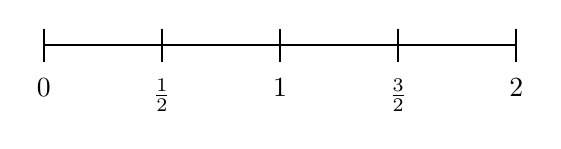
\begin{tikzpicture}[scale=3]
\draw[thick] (0,0) -- (2,0) ; %edit here for the axis
\foreach \x in  {0,0.5,1,1.5,2} % edit here for the vertical lines
\draw[thick, shift={(\x,0)},color=black] (0pt,2pt) -- (0pt,-2pt);
\foreach \n/\texto in {0/{0},.5/{\frac{1}{2}},1/{1},1.5/{\frac{3}{2}},2/{2}}
\node[below] at (\n,-.1) {$\texto$};
\end{tikzpicture}


\uncover<3->{
\[
\int_0^2 \sqrt{1+x^3}dx\approx T_4=\frac{1/2}{2}\left(f(0)+2f(\frac12)+2f(1)+2f(\frac32)+f(2)\right)
\]
}
\uncover<4->{
\[
=\frac14\left(1+2\sqrt{\frac{9}{8}}+2\sqrt{2}+2\sqrt{\frac{35}{8}}+3\right) \approx 3.283
\]
}
\hfill  
%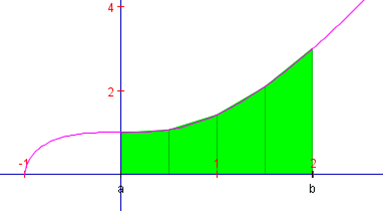
\includegraphics[width=0.3\linewidth]{../../modules/approximate-integration/pictures/Tex1}
} %

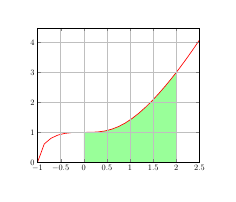
\begin{tikzpicture}[scale=.3]
  \begin{axis}[
    grid=both,
    ymin=0,
    xmin=-1,xmax=2.5,
    axis on top
    ]
    \addplot[draw=none,domain=0:2,fill=green!40] {sqrt(1+x^3)}\closedcycle;
    \addplot[solid,thick,red,domain=-1:2.5] {sqrt(1+x^3)};
  \end{axis}
\end{tikzpicture}


\end{example}
\end{frame}
% % % % % % % % % % % % % % % % % % % % % % % % % % % % % % % %

